%% uncomment to list all files in log
%\listfiles

\documentclass[12pt]{report}


\usepackage{fontspec}

%\setmainfont[Scale=MatchLowercase]{Lucida Bright}
%\setmonofont{FreeMono}
%\setmonofont{Source Code Pro}
\setmonofont[Scale=MatchLowercase]{Ubuntu Mono}

\usepackage[headings]{fullpage}

% national use characters 
%\usepackage{inputenc}

% ams mathematical symbols
\usepackage{amsmath,amssymb}

% added to support pandoc highlighting
\usepackage{microtype}

\usepackage{makeidx}

% add index and bibliographies to table of contents
\usepackage[nottoc]{tocbibind}

% postscript courier and times in place of cm fonts
%\usepackage{courier}
%\usepackage{times}

% extended coloring
\usepackage{color}
\usepackage[table,dvipsnames]{xcolor}
\usepackage{colortbl}

% advanced date formating
\usepackage{datetime}

%support pandoc code highlighting
\usepackage{fancyvrb}
\DefineShortVerb[commandchars=\\\{\}]{\|}
\DefineVerbatimEnvironment{Highlighting}{Verbatim}{commandchars=\\\{\}}
% Add ',fontsize=\small' for more characters per line

%tango style colors
% \usepackage{framed}
% \definecolor{shadecolor}{RGB}{255,255,255}
% \newenvironment{Shaded}{\begin{snugshade}}{\end{snugshade}}
% \newcommand{\KeywordTok}[1]{\textcolor[rgb]{0.13,0.29,0.53}{\textbf{{#1}}}}
% \newcommand{\DataTypeTok}[1]{\textcolor[rgb]{0.13,0.29,0.53}{{#1}}}
% \newcommand{\DecValTok}[1]{\textcolor[rgb]{0.00,0.00,0.81}{{#1}}}
% \newcommand{\BaseNTok}[1]{\textcolor[rgb]{0.00,0.00,0.81}{{#1}}}
% \newcommand{\FloatTok}[1]{\textcolor[rgb]{0.00,0.00,0.81}{{#1}}}
% \newcommand{\CharTok}[1]{\textcolor[rgb]{0.31,0.60,0.02}{{#1}}}
% \newcommand{\StringTok}[1]{\textcolor[rgb]{0.31,0.60,0.02}{{#1}}}
% \newcommand{\CommentTok}[1]{\textcolor[rgb]{0.56,0.35,0.01}{\textit{{#1}}}}
% \newcommand{\OtherTok}[1]{\textcolor[rgb]{0.56,0.35,0.01}{{#1}}}
% \newcommand{\AlertTok}[1]{\textcolor[rgb]{0.94,0.16,0.16}{{#1}}}
% \newcommand{\FunctionTok}[1]{\textcolor[rgb]{0.00,0.00,0.00}{{#1}}}
% \newcommand{\RegionMarkerTok}[1]{{#1}}
% \newcommand{\ErrorTok}[1]{\textbf{{#1}}}
% \newcommand{\NormalTok}[1]{{#1}}

%espresso style colors
% \usepackage{framed}
% \definecolor{shadecolor}{RGB}{42,33,28}
% \newenvironment{Shaded}{\begin{snugshade}}{\end{snugshade}}
% \newcommand{\KeywordTok}[1]{\textcolor[rgb]{0.26,0.66,0.93}{\textbf{{#1}}}}
% \newcommand{\DataTypeTok}[1]{\textcolor[rgb]{0.74,0.68,0.62}{\underline{{#1}}}}
% \newcommand{\DecValTok}[1]{\textcolor[rgb]{0.27,0.67,0.26}{{#1}}}
% \newcommand{\BaseNTok}[1]{\textcolor[rgb]{0.27,0.67,0.26}{{#1}}}
% \newcommand{\FloatTok}[1]{\textcolor[rgb]{0.27,0.67,0.26}{{#1}}}
% \newcommand{\CharTok}[1]{\textcolor[rgb]{0.02,0.61,0.04}{{#1}}}
% \newcommand{\StringTok}[1]{\textcolor[rgb]{0.02,0.61,0.04}{{#1}}}
% \newcommand{\CommentTok}[1]{\textcolor[rgb]{0.00,0.40,1.00}{\textit{{#1}}}}
% \newcommand{\OtherTok}[1]{\textcolor[rgb]{0.74,0.68,0.62}{{#1}}}
% \newcommand{\AlertTok}[1]{\textcolor[rgb]{1.00,1.00,0.00}{{#1}}}
% \newcommand{\FunctionTok}[1]{\textcolor[rgb]{1.00,0.58,0.35}{\textbf{{#1}}}}
% \newcommand{\RegionMarkerTok}[1]{\textcolor[rgb]{0.74,0.68,0.62}{{#1}}}
% \newcommand{\ErrorTok}[1]{\textcolor[rgb]{0.74,0.68,0.62}{\textbf{{#1}}}}
% \newcommand{\NormalTok}[1]{\textcolor[rgb]{0.74,0.68,0.62}{{#1}}}

%kete style colors
% \newenvironment{Shaded}{}{}
% \newcommand{\KeywordTok}[1]{\textbf{{#1}}}
% \newcommand{\DataTypeTok}[1]{\textcolor[rgb]{0.50,0.00,0.00}{{#1}}}
% \newcommand{\DecValTok}[1]{\textcolor[rgb]{0.00,0.00,1.00}{{#1}}}
% \newcommand{\BaseNTok}[1]{\textcolor[rgb]{0.00,0.00,1.00}{{#1}}}
% \newcommand{\FloatTok}[1]{\textcolor[rgb]{0.50,0.00,0.50}{{#1}}}
% \newcommand{\CharTok}[1]{\textcolor[rgb]{1.00,0.00,1.00}{{#1}}}
% \newcommand{\StringTok}[1]{\textcolor[rgb]{0.87,0.00,0.00}{{#1}}}
% \newcommand{\CommentTok}[1]{\textcolor[rgb]{0.50,0.50,0.50}{\textit{{#1}}}}
% \newcommand{\OtherTok}[1]{{#1}}
% \newcommand{\AlertTok}[1]{\textcolor[rgb]{0.00,1.00,0.00}{\textbf{{#1}}}}
% \newcommand{\FunctionTok}[1]{\textcolor[rgb]{0.00,0.00,0.50}{{#1}}}
% \newcommand{\RegionMarkerTok}[1]{{#1}}
% \newcommand{\ErrorTok}[1]{\textcolor[rgb]{1.00,0.00,0.00}{\textbf{{#1}}}}
% \newcommand{\NormalTok}[1]{{#1}}
%end pandoc code hacks

% jodliterate colors
\usepackage{color}
\definecolor{shadecolor}{RGB}{248,248,248}
% j control structures 
\definecolor{keywcolor}{rgb}{0.13,0.29,0.53}
% j explicit arguments x y m n u v
\definecolor{datacolor}{rgb}{0.13,0.29,0.53}
% j numbers - all types see j.xml
\definecolor{decvcolor}{rgb}{0.00,0.00,0.81}
\definecolor{basencolor}{rgb}{0.00,0.00,0.81}
\definecolor{floatcolor}{rgb}{0.00,0.00,0.81}
% j local assignments
\definecolor{charcolor}{rgb}{0.31,0.60,0.02}
\definecolor{stringcolor}{rgb}{0.31,0.60,0.02}
\definecolor{commentcolor}{rgb}{0.56,0.35,0.01}
% primitive adverbs and conjunctions
%\definecolor{othercolor}{rgb}{0.56,0.35,0.01}   
\definecolor{othercolor}{RGB}{0,0,255}
% global assignments
\definecolor{alertcolor}{rgb}{0.94,0.16,0.16}
% primitive J verbs and noun names
\definecolor{funccolor}{rgb}{0.00,0.00,0.00}    

\usepackage{framed}
\newenvironment{Shaded}{}{}
\newcommand{\KeywordTok}[1]{\textcolor{keywcolor}{\textbf{{#1}}}}
\newcommand{\DataTypeTok}[1]{\textcolor{datacolor}{{#1}}}
%\newcommand{\DecValTok}[1]{\textcolor{decvcolor}{{#1}}}
\newcommand{\DecValTok}[1]{{#1}} 
\newcommand{\BaseNTok}[1]{\textcolor{basencolor}{{#1}}}
\newcommand{\FloatTok}[1]{\textcolor{floatcolor}{{#1}}}
\newcommand{\CharTok}[1]{\textcolor{charcolor}{\textbf{{#1}}}}
\newcommand{\StringTok}[1]{\textcolor{stringcolor}{{#1}}}
\newcommand{\CommentTok}[1]{\textcolor{commentcolor}{\textit{{#1}}}}
\newcommand{\OtherTok}[1]{\textcolor{othercolor}{{#1}}} 
\newcommand{\AlertTok}[1]{\textcolor{alertcolor}{\textbf{{#1}}}}
%\newcommand{\FunctionTok}[1]{\textcolor{funccolor}{{#1}}}
\newcommand{\FunctionTok}[1]{{#1}}
\newcommand{\RegionMarkerTok}[1]{{#1}}
\newcommand{\ErrorTok}[1]{\textbf{{#1}}}
\newcommand{\NormalTok}[1]{{#1}}

% headers and footers
\usepackage{fancyhdr}
\pagestyle{fancy}

\fancyhead{}
\fancyfoot{}

%\fancyhead[LE,RO]{\slshape \rightmark}
%\fancyhead[LO,RE]{\slshape \leftmark}
\fancyfoot[C]{\thepage}
%\headrulewidth 0.4pt
%\footrulewidth 0 pt

%\addtolength{\headheight}{\baselineskip}

%\lfoot{\emph{Analyze the Data not the Drivel}}
%\rfoot{\emph{\today}}

% subfigure handles figures that contain subfigures
%\usepackage{color,graphicx,subfigure,sidecap}
\usepackage{graphicx,sidecap}
\usepackage{subfigure}
\graphicspath{{./inclusions/}}

% floatflt provides for text wrapping around small figures and tables
\usepackage{floatflt}

% tweak caption formats 
\usepackage{caption} 
\usepackage{sidecap}
%\usepackage{subcaption} % not compatible with subfigure

\usepackage{rotating} % flip tables sideways

% complex footnotes
%\usepackage{bigfoot}

% weird logos \XeLaTeX
\usepackage{metalogo}

% source code listings
\usepackage{listings}

% long tables
% \usepackage{longtable}

\newcommand{\HRule}{\rule{\linewidth}{0.5mm}}

% map LaTeX cross references into PDF cross references
\usepackage[
            %dvips,
            colorlinks,
            linkcolor=blue,
            citecolor=blue,
            urlcolor=blue,   % magenta, cyan default        
            pdfauthor={John D. Baker},
            pdftitle={Analyze the Data not the Drivel},
            pdfsubject={Blog},
            pdfcreator={MikTeX+LaTeXe with hyperref package},
            pdfkeywords={blog,wordpress},
            ]{hyperref}
           
% custom colors
\definecolor{CodeBackGround}{cmyk}{0.0,0.0,0,0.05}    % light gray
\definecolor{CodeComment}{rgb}{0,0.50,0.00}           % dark green {0,0.45,0.08}
\definecolor{TableStripes}{gray}{0.9}                 % odd/even background in tables

\lstdefinelanguage{bat}
{morekeywords={echo,title,pushd,popd,setlocal,endlocal,off,if,not,exist,set,goto,pause},
sensitive=True,
morecomment=[l]{rem}
}

\lstdefinelanguage{jdoc}
{
morekeywords={},
otherkeywords={assert.,break.,continue.,for.,do.,if.,else.,elseif.,return.,select.,end.
,while.,whilst.,throw.,catch.,catchd.,catcht.,try.,case.,fcase.},
sensitive=True,
morecomment=[l]{NB.},
morestring=[b]',
morestring=[d]',
}

% latex size ordering - can never remember it
% \tiny
% \scriptsize
% \footnotesize
% \small
% \normalsize
% \large
% \Large
% \LARGE
% \huge
% \Huge
 
% listings package settings  
\lstset{%
  language=jdoc,                                % j document settings
  basicstyle=\ttfamily\footnotesize,            
  keywordstyle=\bfseries\color{keywcolor}\footnotesize,
  identifierstyle=\color{black},
  commentstyle=\slshape\color{CodeComment},     % colored slanted comments
  stringstyle=\color{red}\ttfamily,
  showstringspaces=false,                       
  %backgroundcolor=\color{CodeBackGround},       
  frame=single,                                
  framesep=1pt,                                 
  framerule=0.8pt,                             
  rulecolor=\color{CodeBackGround},   
  showspaces=false,
  %columns=fullflexible,
  %numbers=left,
  %numberstyle=\footnotesize,
  %numbersep=9pt,
  tabsize=2,
  showtabs=false,
  captionpos=b
  breaklines=true,                              
  breakindent=5pt                              
}

\lstdefinelanguage{JavaScript}{
  keywords={typeof, new, true, false, catch, function, return, null, catch, switch, var, if, in, while, do, else, case, break},
  ndkeywords={class, export, boolean, throw, implements, import, this},
  ndkeywordstyle=\color{darkgray}\bfseries,
  sensitive=false,
  comment=[l]{//},
  morecomment=[s]{/*}{*/},
  morestring=[b]',
  morestring=[b]"
}

% C# settings
\lstdefinestyle{sharpc}{
language=[Sharp]C,
basicstyle=\ttfamily\scriptsize, 
keywordstyle=\bfseries\color{keywcolor}\scriptsize,
framerule=0pt
}

% for source code listing longer than two use smaller font
\lstdefinestyle{smallersource}{
basicstyle=\ttfamily\scriptsize, 
keywordstyle=\bfseries\color{keywcolor}\scriptsize,
framerule=0pt
}

\lstdefinestyle{resetdefaults}{
language=jdoc,
basicstyle=\ttfamily\footnotesize,  
keywordstyle=\bfseries\color{keywcolor}\footnotesize,                                                               
framerule=0.8pt 
}

% APL UTF8 code points listed for lstlisting processing
\makeatletter
\lst@InputCatcodes
\def\lst@DefEC{%
 \lst@CCECUse \lst@ProcessLetter
  ^^80^^81^^82^^83^^84^^85^^86^^87^^88^^89^^8a^^8b^^8c^^8d^^8e^^8f%
  ^^90^^91^^92^^93^^94^^95^^96^^97^^98^^99^^9a^^9b^^9c^^9d^^9e^^9f%
  ^^a0^^a1^^a2^^a3^^a4^^a5^^a6^^a7^^a8^^a9^^aa^^ab^^ac^^ad^^ae^^af%
  ^^b0^^b1^^b2^^b3^^b4^^b5^^b6^^b7^^b8^^b9^^ba^^bb^^bc^^bd^^be^^bf%
  ^^c0^^c1^^c2^^c3^^c4^^c5^^c6^^c7^^c8^^c9^^ca^^cb^^cc^^cd^^ce^^cf%
  ^^d0^^d1^^d2^^d3^^d4^^d5^^d6^^d7^^d8^^d9^^da^^db^^dc^^dd^^de^^df%
  ^^e0^^e1^^e2^^e3^^e4^^e5^^e6^^e7^^e8^^e9^^ea^^eb^^ec^^ed^^ee^^ef%
  ^^f0^^f1^^f2^^f3^^f4^^f5^^f6^^f7^^f8^^f9^^fa^^fb^^fc^^fd^^fe^^ff%
  ^^^^20ac^^^^0153^^^^0152%
  ^^^^20a7^^^^2190^^^^2191^^^^2192^^^^2193^^^^2206^^^^2207^^^^220a%
  ^^^^2218^^^^2228^^^^2229^^^^222a^^^^2235^^^^223c^^^^2260^^^^2261%
  ^^^^2262^^^^2264^^^^2265^^^^2282^^^^2283^^^^2296^^^^22a2^^^^22a3%
  ^^^^22a4^^^^22a5^^^^22c4^^^^2308^^^^230a^^^^2336^^^^2337^^^^2339%
  ^^^^233b^^^^233d^^^^233f^^^^2340^^^^2342^^^^2347^^^^2348^^^^2349%
  ^^^^234b^^^^234e^^^^2350^^^^2352^^^^2355^^^^2357^^^^2359^^^^235d%
  ^^^^235e^^^^235f^^^^2361^^^^2362^^^^2363^^^^2364^^^^2365^^^^2368%
  ^^^^236a^^^^236b^^^^236c^^^^2371^^^^2372^^^^2373^^^^2374^^^^2375%
  ^^^^2377^^^^2378^^^^237a^^^^2395^^^^25af^^^^25ca^^^^25cb%  
  ^^00}
\lst@RestoreCatcodes
\makeatother

% custom lengths used within minipages
\newcommand{\minindent}{17pt}


\makeindex

\begin{document}

\subsection*{\href{https://bakerjd99.wordpress.com/2011/02/12/j-7-01-now-playing-in-your-browser/}{J 7.01 Now Playing in your Browser}}
\addcontentsline{toc}{subsection}{J 7.01 Now Playing in your Browser}


\noindent\emph{Posted: 12 Feb 2011 22:01:31}
\vspace{6pt}

Big changes are afoot for J programmers. With the release of
\href{http://www.jsoftware.com/docs/help701/user/relhigh.htm}{J 7.01}
\href{http://www.jsoftware.com/}{JSOFTWARE} has taken the risky step of
\href{http://en.wikipedia.org/wiki/Deprecation}{deprecating} two well
established user
\href{http://en.wikipedia.org/wiki/Integrated\_development\_environment}{IDE's}
and replacing them with brand new \href{http://www.gtk.org/}{GTK} and
Web browser-based interfaces. As we all know new software is not
necessarily better software, (remember that risky bit), but in this case
the changes make sense.


%{[}caption id=``'' align=``aligncenter'' width=``482'' caption=``J 7.01  running JHS on  Chrome''{]}
%\href{http://bakerjd99.files.wordpress.com/2011/02/j701chrome.png}{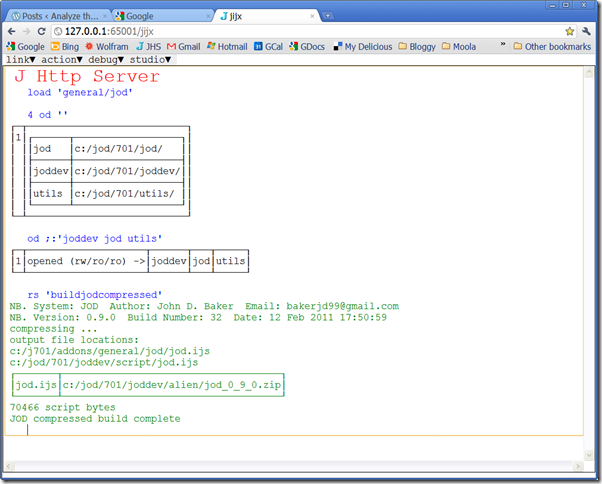
\includegraphics{j701chrome_thumb.png}}
%{[}/caption{]}
\captionsetup[figure]{labelformat=empty}
\begin{figure}[htbp]
\centering
\href{http://www.jsoftware.com/}{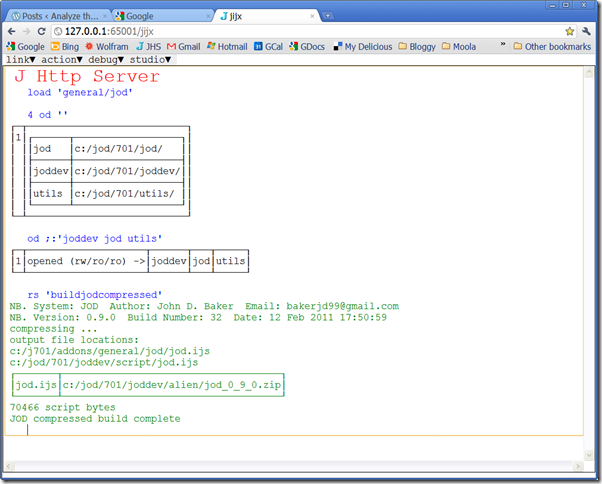
\includegraphics[width=0.60\textwidth]{j701chrome_thumb.png}}
\caption{J 7.01  running JHS on  Chrome}
\label{fig:1070X0}
\end{figure}


Early J systems were largely Windows-Centric. Yes, J has run perfectly
well on strains of UNIX/Linux and the Mac for over a decade but I think
it's fair to say that J IDE's were biased toward Windows. JSOFTWARE was
well aware of this and tried to offer the features of their Windows IDE
with a portable Java based IDE. Unfortunately the Java IDE, like Java
itself, failed to live up to expectations.

Now that the many, if not the majority of J programmers, run J on
non-Windows, (mostly Linux and the Mac), systems it makes no sense to
treat them like second class citizens. So how do you provide a
\emph{state of the art portable user IDE} that runs well on Windows,
Linux, the Mac, smart phones and various
\href{http://pinoytutorial.com/techtorial/iboard-and-imat-future-of-apple-products/}{IGadgets}.
There is no single answer so JSOFTWARE wisely decided to offer two IDEs:
JHS and
\href{http://www.jsoftware.com/jwiki/System/Installation/J701/Gtk}{JGTK}.

The JGTK IDE is a desktop application that is similar to the older
Windows IDE. JGTK is somewhat biased toward Linux but this his doesn't
mean it doesn't work well on other systems. I run it on WinXP and Win7
machines all the time. JGTK takes longer to load than the older Windows
IDE but once it's up and running I don't see significant performance
differences. The JGTK editor is superior to the older Windows editor and
I love the side bar and UNIX style code tagging. For a first version
JGTK is a nice bit of work that will only improve as J programmers and
users pound away on it.

JGTK is nice but JHS is radical. JHS abandons the desktop and turns your
favorite web browser into a stripped down J programming environment. I
was skeptical when I first heard about JHS but it has won me over. JHS
is amazingly effective under Google's Chrome browser. It comes up in a
flash and is as zippy or faster than the older Windows IDE. Even better
this webby goodness imposes minimal burdens. The JHS web server is often
one of the smaller processes running on my machines. I have been doing
the bulk of my
\href{https://github.com/bakerjd99/jod/blob/master/joddocument/pdfdoc/jod.pdf}{JOD}
update work with JHS and I frequently forget I'm using a browser!
\emph{Good user
interfaces,} \emph{\href{http://www.nationalreview.com/articles/225959/coming-obama-thugocracy/michael-barone}{unlike
politicians}}\emph{, get out of your face!}

As for my \href{http://www.jsoftware.com/jwiki/Addons/general/jod}{J
addon JOD}: J 7.01 introduced a number of system script changes that
break JOD 0.8.0. I am working on JOD 0.9.0, (a beta version is available
in the files box sidebar of this blog), that fixes these problems and
implements some planned changes. The biggest change so far: I have moved
the JOD interface out of the \textbf{z} locale into it's own
\textbf{ijod} interface locale. How's this for a marketing slogan?
\textbf{JOD 0.9.x -- now with less z stomping!}

%\captionsetup[floatingfigure]{labelformat=empty}
%\begin{figure}[htbp]
%\begin{floatingfigure}[l]{0.25\textwidth}
%\centering
%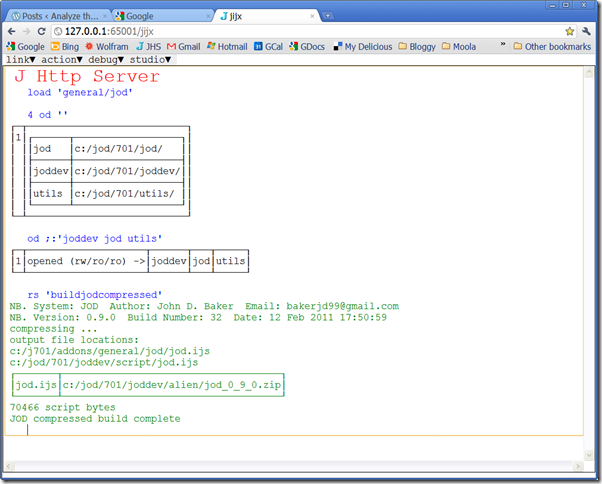
\includegraphics[width=0.23\textwidth]{j701chrome_thumb.png}
%\caption{~~~IMCAPTION~~~}
%\label{fig:1070X0}
%\end{floatingfigure}
%\end{figure}



%\end{document}